\newcommand{\req}[1]{RQ#1}

\section{Evaluation}\label{sec:eval}

\begin{table}[t]
%  \vspace{2mm}
  \caption{Analysis results of NativeFlowBench}
  \label{table:RQ1-1}
  \vspace*{-1em}
  \centering
%  \footnotesize
\renewcommand{\arraystretch}{.9}
  \begin{tabular}{l||c|c}
\multicolumn{1}{c||}{\textbf{Benchmark}} & \textbf{\jnsaf} & \textbf{\ours}\\\hline\hline
    icc\_javatonative                   & $\bigcirc$ & $\times$\\
    icc\_nativetojava                   & $\bigcirc$ & $\times$\\
    native\_complexdata                 & $\bigcirc$ & $\bigcirc$\\
    native\_complexdata\_stringop       & $\times$ & $\times$\\
    native\_dynamic\_register\_multiple & $\bigcirc$ & $\bigcirc$\\
    native\_heap\_modify                & $\bigcirc$ & $\bigcirc$\\
    native\_leak                        & $\bigcirc$ & $\bigcirc$\\
    native\_leak\_array                 & $\bigcirc$ & $\times$\\
    native\_leak\_dynamic\_register     & $\bigcirc$ & $\bigcirc$\\
    native\_method\_overloading         & $\bigcirc$ & $\bigcirc$\\
    native\_multiple\_interactions      & $\bigcirc$ & $\bigcirc$\\
    native\_multiple\_libraries         & $\bigcirc$ & $\bigcirc$\\
 native\_noleak                       & $\bigcirc$ & $\bigcirc$ \\
 native\_noleak\_array                & $\times$ & $\bigcirc$  \\
 native\_nosource                     & $\bigcirc$ & $\bigcirc$  \\
 native\_pure                         & $\bigcirc$ & $\bigcirc$  \\
 native\_pure\_direct                 & $\bigcirc$ & $\bigcirc$  \\
 native\_pure\_direct\_customized     & $\bigcirc$ & $\bigcirc$  \\
 native\_set\_field\_from\_arg        & $\bigcirc$ & $\bigcirc$  \\
 native\_set\_field\_from\_arg\_field & $\bigcirc$ & $\bigcirc$  \\
 native\_set\_field\_from\_native     & $\bigcirc$ & $\bigcirc$  \\
 native\_source                       & $\bigcirc$ & $\bigcirc$  \\
 native\_source\_clean                & $\bigcirc$ & $\bigcirc$
  \end{tabular}
\vspace*{-1em}
\end{table}



To show the effectiveness of our approach, we evaluate
\ours with the following two research questions:
\begin{itemize}
  \item \textbf{\req{1}: Feasibility.} Does \ours correctly analyze multilingual
    programs that use various interoperations?

  \item \textbf{\req{2}: Usefulness.} Does \ours correctly detect dataflow-related
    bugs?
%that the state-of-the-art multilingual program analyzers detect?
\end{itemize}

\subsection{\req{1}: Feasibility}
We evaluate the feasibility of \ours by dataflow analysis on
two benchmark suites for each of Java-C and Python-C analyses.

\subsubsection{Feasibility: Java-C}
The first benchmark suite for Java-C program analysis is NativeFlowBench~\cite{nativeflowbench, JN-SAF},
consisting of 23 JNI Android applications (apps) that use various JNI interoperations.
They contain sensitive data leakage from {\it sources} to {\it sinks}
across language boundaries via JNI interoperations.
We compare the analysis results of \ours to those of the state-of-the-art Java-C program
dataflow analyzer, \jnsaf~\cite{JN-SAF}. We use
compiled versions for \jnsaf because it targets compiled JNI programs.

Table~\ref{table:RQ1-1} summarizes the analysis
results of \jnsaf and \ours on NativeFlowBench.
{\bf Benchmark} columns show the benchmark names
and {\bf JN-SAF} and {\bf MultiQL} columns show 
the analysis results of \jnsaf and \ours, respectively.
If an analysis reports all data leakages correctly without any
false positives or false negatives, it is a success (\cmark).
Otherwise, it is a failure (\xmark).
\ours finds data leakages correctly for 19 benchmarks but reports false
negatives for four benchmarks, while \jnsaf analyzes 21 benchmarks correctly. 
One common failure comes from string concatenation:
{\it native\_complexdata\_stringop} generates a Java field name by
concatenating two string values via a built-in function.
Because \ours does not handle built-in functions, it fails to analyze the benchmark.
{\it icc\_javatonative} and {\it icc\_nativetojava} leak data via the Android
inter-component communication, which is beyond the scope of \ours.
The remaining different failures of \ours and \jnsaf come from
their different array analysis policies.
While both {\it native\_leak\_array} and {\it native\_noleak\_array} store sensitive data in an array,
the former leaks the data, but the latter does not.
Because \jnsaf over-approximates dataflows on arrays,
it analyzes {\it native\_leak\_array} correctly but reports a false positive for {\it native\_noleak\_array}.
On the contrary, because CodeQL under-approximates dataflows on arrays,
\ours analyzes {\it native\_noleak\_array} correctly but reports a false negative for
{\it native\_leak\_array}.
%
The results show that \ours can successfully analyze JNI programs that
use various JNI interoperations, and its correctness is comparable with that of \jnsaf.

%\textbf{Real-world Java-C Programs.} 
The second benchmark suite consists of real-world Java-C Android apps downloaded from
F-Droid, a repository of open-source Android apps~\cite{fdroid}.  We first
downloaded all available apps from F-Droid, and classified downloaded apps into JNI and non-JNI apps.
Then, we selected all 42 apps that can be compiled without any errors as our analysis targets.
For this real-world benchmark, we compare the analysis results of
\ours to those of \lees~\cite{LeeASE20},
the state-of-the-art general-purpose Java-C program analyzer.
We use \lees as a comparison target instead of \jnsaf,
since \jnsaf is not scalable enough to analyze the real-world benchmark.

\begin{table*}[t]
%  \vspace{2mm}
  \caption{Analysis results of real-world Android JNI applications}
  \label{table:RQ1-2}
  \vspace*{-.5em}
  \centering
  \footnotesize
%\renewcommand{\arraystretch}{.9}
  \begin{tabular}{@{}l||r|r|r|r|r||r|r|r||r|r|r@{}}
    \multirow{3}{*}{\textbf{Application}} & \multicolumn{5}{c||}{\textbf{Time (sec.)}} & \multicolumn{3}{c||}{\multirow{2}{*}{\textbf{C->Java Function Call}}} & \multicolumn{3}{c}{\multirow{2}{*}{\textbf{C->Java Field Access}}} \\\hhline{~||-----||~~~||~~~}
    & \multicolumn{3}{c|}{\textbf{DB Creation}} & \multicolumn{1}{c|}{\multirow{2}{*}{\textbf{Query}}} & \multicolumn{1}{c||}{\multirow{2}{*}{\textbf{Total}}} & \multicolumn{3}{c||}{} & \multicolumn{3}{c}{} \\\hhline{~||---~|~||------}
    & \multicolumn{1}{c|}{\textbf{C}} & \multicolumn{1}{c|}{\textbf{Java}} & \multicolumn{1}{c|}{\textbf{Merged}} & \multicolumn{1}{c|}{} & \multicolumn{1}{c||}{} & \multicolumn{1}{c|}{\textbf{\# Precise}} & \multicolumn{1}{c|}{\textbf{\# Resolved}} & \multicolumn{1}{c||}{\textbf{Total}} & \multicolumn{1}{c|}{\textbf{\# Precise}} & \multicolumn{1}{c|}{\textbf{\# Resolved}} & \multicolumn{1}{l}{\textbf{Total}}  \\\hhline{=#*{4}{=|}=#=|=|=#=|=|=}
  1. Agram                  & 2.538                 & 5.002                    & 3.643                      & 6.829                                      & 18.012                                  & 0                           & 0                            & 2                         & 4                           & 4                            & 4                          \\
  2. AndIodine              & 2.805                 & 8.237                    & 3.989                      & 8.114                                      & 23.145                                  & 1                           & 1                            & 1                         & 0                           & 0                            & 0                          \\
  3. APV PDF Viewer         & 56.496                & 9.252                    & 23.349                     & 35.688                                     & 124.785                                 & 4                           & 4                            & 4                         & 15                          & 15                           & 16                         \\
  4. CommonsLab             & 23.176                & 24.139                   & 14.149                     & 20.554                                     & 82.018                                  & 4                           & 5                            & 5                         & 0                           & 0                            & 0                          \\
  5. CrossWords             & 29.754                & 21.663                   & 23.276                     & 29.106                                     & 103.799                                 & 68                          & 68                           & 70                        & 9                           & 10                           & 14                         \\
  6. Document Viewer        & 180.71                & 20.292                   & 56.743                     & 75.934                                     & 333.679                                 & 6                           & 6                            & 6                         & 23                          & 23                           & 24                         \\
  7. DroidZebra             & 17.774                & 7.141                    & 5.817                      & 12.608                                     & 43.34                                   & 4                           & 5                            & 5                         & 0                           & 0                            & 0                          \\
  8. FBReader               & 85.398                & 27.114                   & 36.36                      & 30.072                                     & 178.944                                 & 0                           & 0                            & 0                         & 0                           & 0                            & 1                          \\
  9. Fwknop2                & 11.834                & 11.488                   & 7.395                      & 10.446                                     & 41.163                                  & 0                           & 0                            & 0                         & 0                           & 13                           & 13                         \\
  10. Graph 89               & 72.609                & 8.47                     & 41.465                     & 598.645                                    & 721.189                                 & 1                           & 1                            & 1                         & 0                           & 0                            & 0                          \\
  11. Irssi ConnectBot       & 1.284                 & 12.32                    & 6.048                      & 11.196                                     & 30.848                                  & 1                           & 1                            & 1                         & 0                           & 0                            & 2                          \\
  12. Lumicall               & 40.486                & 13.102                   & 17.328                     & 27.104                                     & 98.02                                   & 4                           & 4                            & 4                         & 2                           & 2                            & 13                         \\
  13. Navit                  & 26.761                & 17.741                   & 54.751                     & 46.264                                     & 145.517                                 & 16                          & 22                           & 55                        & 0                           & 0                            & 0                          \\
  14. NetGuard               & 14.958                & 16.925                   & 9.988                      & 12.716                                     & 54.587                                  & 0                           & 9                            & 9                         & 3                           & 27                           & 27                         \\
  15. Overchan               & 1.727                 & 22.043                   & 8.772                      & 15.143                                     & 47.685                                  & 1                           & 2                            & 4                         & 0                           & 0                            & 1                          \\
  16. Plumble                & 28.501                & 12.365                   & 16.335                     & 29.253                                     & 86.454                                  & 0                           & 0                            & 0                         & 610                         & 610                          & 610                        \\
  17. PrBoom                 & 48.312                & 5.469                    & 21.601                     & 32.001                                     & 107.383                                 & 7                           & 7                            & 15                        & 0                           & 0                            & 0                          \\
  18. Rtl-sdr driver         & 18.797                & 16.984                   & 9.623                      & 11.751                                     & 57.155                                  & 2                           & 2                            & 2                         & 0                           & 0                            & 0                          \\
  19. Sipdroid               & 20.267                & 11.864                   & 10.961                     & 18.577                                     & 61.669                                  & 2                           & 2                            & 2                         & 2                           & 2                            & 16                         \\
  20. Son of Hunky Punk      & 40.266                & 14.947                   & 20.582                     & 31.102                                     & 106.897                                 & 50                          & 50                           & 52                        & 10                          & 10                           & 10                         \\
  21. Taps Of Fire           & 3.566                 & 7.521                    & 4.453                      & 8.145                                      & 23.685                                  & 0                           & 0                            & 0                         & 2                           & 2                            & 2                          \\
  22. Tileless Map           & 273.993               & 187.099                  & 118.557                    & 146.806                                    & 726.455                                 & 50                          & 58                           & 59                        & 3                           & 4                            & 5                          \\
  23. Timidity AE            & 23.417                & 11.718                   & 13.03                      & 28.452                                     & 76.617                                  & 16                          & 16                           & 16                        & 0                           & 0                            & 0                          \\
  24. Tux Paint              & 256.126               & 120.831                  & 161.906                    & 184.591                                    & 723.454                                 & 80                          & 83                           & 89                        & 4                           & 4                            & 6                          \\
  25. VotAR                  & 1.515                 & 5.189                    & 3.569                      & 6.532                                      & 16.805                                  & 1                           & 1                            & 2                         & 3                           & 3                            & 3                          \\\hhline{=#*{4}{=}=#=|=|=#=|=|=}
    \textbf{Total}       & \multicolumn{1}{r}{}  & \multicolumn{1}{r}{}     & \multicolumn{1}{r}{}       & \multicolumn{1}{r}{}                       & \multicolumn{1}{r||}{}                    & 318                         & 347                          & 404                       & 690                         & 729                          & 767
  \end{tabular}
\end{table*}


\begin{figure}
  \centering
  \vspace{2mm}
  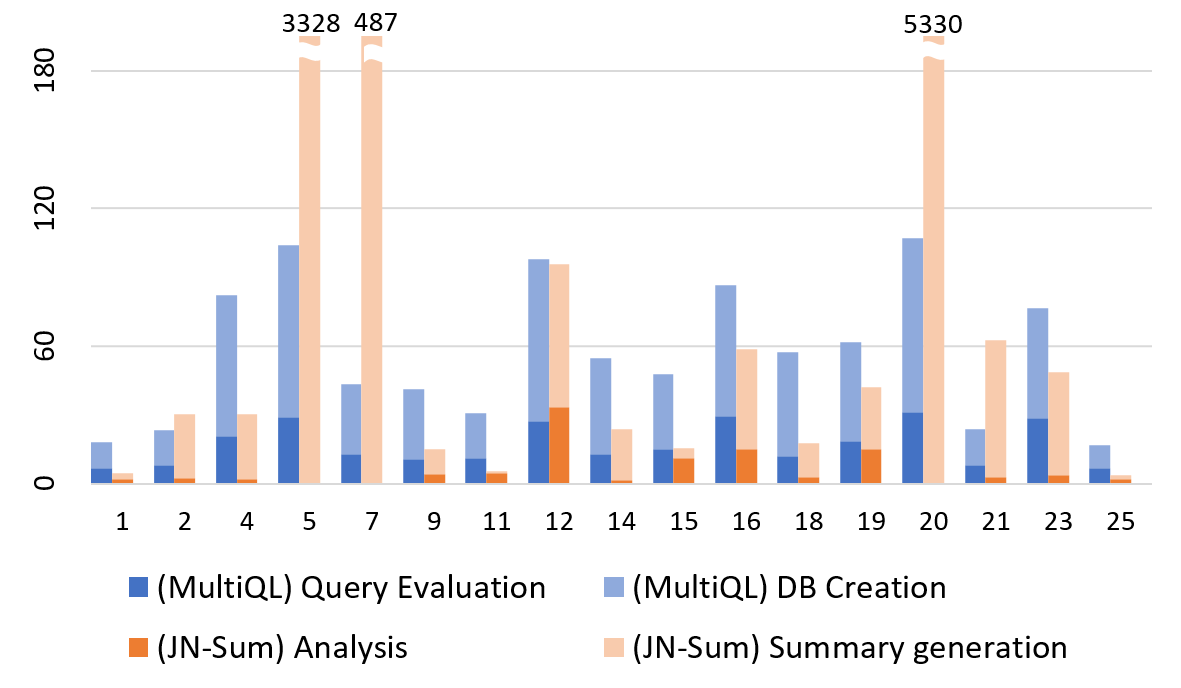
\includegraphics[width=0.65\textwidth]{img/graph}
  \vspace*{-.5em}
  \caption{Analysis time of \ours and \lees}
  \label{fig:graph}
\vspace*{-1em}
\end{figure}

Table~\ref{table:RQ1-2} shows the analysis results of \ours on 25 apps that have
interoperations from C to Java.
The first column shows app names with their indices, the second shows the lines of code,
the third shows database creation time, the
fourth shows query processing time, and the fifth shows the total analysis time.
{\bf C->Java Function Call} and {\bf C->Java Field Access} show the numbers of
C-to-Java function calls and C-to-Java field accesses, respectively. We
collectively call them \emph{JNI uses}.
The sub-columns {\bf \#Precise}, {\bf \#Resolved}, and {\bf Total} represent
the numbers of precisely resolved, resolved, and the total JNI uses,
respectively.
We considered a resolved JNI use as precise, when \ours finds a single target
method or a single field at the JNI use.
\ours resolves 1,076 out of 1,171 (92\%) JNI uses, including 347 out of 404
(86\%) C-to-Java function calls and 729 out of 767 (95\%) C-to-Java field
accesses. 
In addition, 1,008 (86\%) resolved JNI uses are precise.
\ours fails to resolve 95 (8\%) JNI uses because of complex language semantics
such as arrays and function pointers, on which
CodeQL does not track dataflows.

On the contrary,
\lees fails to analyze one app because of an error, four apps due to the lack
of memory spaces, and three apps even in eight hours.  
In the remaining 17 apps, \lees resolves 71\% JNI uses
and precisely resolves 46\% of JNI uses,
which shows significantly more imprecise results than \ours.

\ours is scalable in that it can analyze large-scale programs. 
The analysis time was 161.3 seconds on average for each app, including 103.8
seconds for DB creation and 57.5 seconds for query processing.  
DB creation took more time than query processing except for {\it Graph 89}, and
the DB creation time was almost linear to the code size. 
\ours took about 12 minutes at most to analyze {\it Tileless Map} having about
one million lines of code.

Figure~\ref{fig:graph} shows the analysis time of \ours compared to \lees.
The x-axis denotes the indices of apps and the y-axis denotes the analysis time
in seconds. We omit eight apps \lees fails to analyze.
\lees analyzes 12 apps faster than \ours, but the difference is less than two
minutes. 
On the other hand, \ours analyzes five apps faster than \lees, and \lees spends
much time in summary generation for three apps among them. 
In addition, while \lees fails to analyze all the large-scale apps that have
more than about 400,000 lines of code in eight hours, \ours analyzes about
three million lines of code in about 12 minutes.

In summary, the evaluation with the second benchmark suite shows that
\ours can analyze real-world JNI applications more precisely than \lees.
In addition, the scalability of \ours is comparable with \lees in that
it can analyze larger apps much faster than \lees.

\subsubsection{Feasibility: Python-C}
\begin{table}[t]
%  \vspace{2mm}
  \caption{Analysis results of ExtModuleFlowBench}
  \label{table:RQ1-3}
  \vspace*{-1em}
  \centering
%  \footnotesize
\renewcommand{\arraystretch}{.9}
  \begin{tabular}{l|c||l|c}
    \textbf{Benchmark} & \textbf{Dataflow} & \textbf{Benchmark} & \textbf{Dataflow}
%\\\hline\hline
\\\hhline{=|=#=|=}
    callback                    & \cmark & multiple\_module             & \cmark \\
    cobject\_member             & \cmark & noleak                       & \cmark \\
    cobject\_method             & \cmark & noleak\_array                & \cmark \\
    complexdata                 & \cmark & nosource                     & \cmark \\
    complexdata\_stringop       & \xmark & parse\_arg                   & \cmark \\
    heap\_modify                & \cmark & set\_field\_from\_arg        & \xmark \\
    import\_module              & \cmark & set\_field\_from\_arg\_field & \xmark \\
    leak                        & \cmark & set\_field\_from\_native     & \xmark \\
    leak\_array                 & \xmark & source                       & \cmark \\
    multiple\_interactions      & \cmark & source\_clean                & \xmark
  \end{tabular}
\end{table}


The first benchmark suite for Python-C program analysis is ExtModuleFlowBench we developed,
consisting of 20 Python-C programs.
We converted each Java-C benchmark in NativeFlowBench into a
corresponding Python-C program, except for eight apps containing JNI-specific interoperation
features. Additionally, we made five Python-C programs that contain interoperations
specific to Python Extension Module.

Table~\ref{table:RQ1-3} summarizes the analysis results of \ours
on 20 Python-C programs in ExtModuleFlowBench.
{\bf Benchmark} columns show the benchmark names and {\bf Dataflow}
columns show the analysis results.
\ours analyzes dataflows correctly for 14 benchmarks, but reports false
negatives for six benchmarks.
\ours fails in {\it complexdata\_stringop} and {\it leak\_array} due to the
same reason for NativeFlowBench.
For the other four benchmarks, \ours fails to track dataflows for the fields of Python objects. 
In the failed benchmarks, the C code changes the values of the fields in Python objects that are passed
to the parameters of C functions.
\ours does not handle such cases because
the use of a virtual argument node prevents the propagation of changed values
back to the field of the original Python object, and it
reports false negatives for them.
The results show that our approach can analyze Python-C programs using various interoperations,
just like it can analyze JNI programs using various JNI interoperations.

\begin{table}[t]
%  \vspace{2mm}
  \caption{Analysis results of real-world extension modules}
  \label{table:RQ1-4}
  \vspace*{-1em}
  \centering
%  \footnotesize
\renewcommand{\arraystretch}{.9}
\begin{tabular}{@{}l@{~}| %Repository
 @{~}r@{~}|@{~}r@{~}|@{~}r@{~}|@{~}r@{~}|@{~}r@{~}|@{~}r@{~}|@{~}r@{}}
\multicolumn{1}{@{}l|@{~}}{\multirow{2}{*}{\textbf{Repository}}}
 & \multicolumn{3}{@{~}c|@{~}}{\textbf{DB Creation (sec.)}}
 & \multicolumn{1}{@{~}c|@{~}}{\textbf{Query}}
 & \multicolumn{1}{@{~}c|@{~}}{\textbf{Total}}
 & \multicolumn{2}{@{~}c@{}}{\textbf{\# API calls}}
%\\\hhline{~|---~|~|--}
%\\\cline{2-4}\cline{7-8}
\\
\multicolumn{1}{@{}l|@{~}}{}
 & \multicolumn{1}{@{~}c|@{~}}{\textbf{Python}}
 & \multicolumn{1}{@{~}c|@{~}}{\textbf{C}}
 & \multicolumn{1}{@{~}c|@{~}}{\textbf{Merged}}
 & \multicolumn{1}{@{~}c|@{~}}{\textbf{(sec.)}}
 & \multicolumn{1}{@{~}c|@{~}}{\textbf{(sec.)}}
 & \multicolumn{1}{@{~}c|@{~}}{\textbf{Res.}}
 & \multicolumn{1}{c@{}}{\textbf{Total}}
% %\\\hhline{=#*{4}{=|}=#=|=}
\\\hline\hline
  % 1. bitarray           & 19.378 & 3.082 & 13.537 & 197.556 & 233.553 & 38 & 50 \\
  % 2. distance           & 16.722 & 2.354 & 11.594 & 134.895 & 165.565 & -  & -  \\
  % 3. noise              & 18.79  & 2.43  & 12.222 & 148.021 & 181.463 & -  & -  \\
  % 4. pyahocorasick      & 19.179 & 2.62  & 13.118 & 172.62  & 207.537 & 33 & 43 \\
  % 5. python-Levenshtein & 17.187 & 3.144 & 12.686 & 153.95  & 186.967 & -  & -  \\
  % 6. python-llist       & 17.047 & 2.853 & 11.986 & 153.014 & 184.9   & 18 & 30 \\\hhline{=#*{4}{=}=#=|=}
\multicolumn{1}{@{}l|@{~}}{bitarray}
           & 19.378 & 3.082 & 13.537 & 197.556 & 233.553 & 38 & 50 \\
\multicolumn{1}{@{}l|@{~}}{distance}
           & 16.722 & 2.354 & 11.594 & 134.895 & 165.565 & -  & -  \\
\multicolumn{1}{@{}l|@{~}}{noise}
            & 18.790  & 2.430  & 12.222 & 148.021 & 181.463 & -  & -  \\
\multicolumn{1}{@{}l|@{~}}{pyahocorasick}
      & 19.179 & 2.620  & 13.118 & 172.620  & 207.537 & 33 & 43 \\
\multicolumn{1}{@{}l|@{~}}{python-Levenshtein} & 17.187 & 3.144 & 12.686 & 153.950  & 186.967 & -  & -  \\
\multicolumn{1}{@{}l|@{~}}{python-llist}       & 17.047 & 2.853 & 11.986 & 153.014 & 184.900   & 18 & 30
%\\\hhline{=#*{4}{=}=#=|=}
\\\hline\hline
\multicolumn{1}{@{}l|@{~}}{\textbf{Total}}
 & \multicolumn{1}{r}{}
 & \multicolumn{1}{r}{}
 & \multicolumn{1}{r}{}
 & \multicolumn{1}{r}{}
 & \multicolumn{1}{r|@{~}}{}
 & 89                         & 123                          
  \end{tabular}
\vspace*{-1em}
\end{table}


%\textbf{Github}
%\textbf{Real-world Python-C Programs.}
The second benchmark suite consists of six real-world Python-C programs
collected from public GitHub repositories. They are analysis targets of
Monat et al.~\cite{sas2021}'s work.

Table~\ref{table:RQ1-4} summarizes the dataflow analysis results on six
real-world Python-C programs. 
The first column shows repository names, the second shows the lines of code,
the third shows database creation time,
the fourth shows query processing time, the fifth shows the total analysis time,
and the last two columns denote analysis results.
{\bf \#~Resolved} column denotes the number of resolved API function calls in C code and
{\bf Total} column denotes the total number of Python Extension Module API function
calls in C code. 
Because all the API functions take a Python object as the first argument, we
considered an API function call as resolved, when \ours finds its first argument
correctly. 


Out of six programs, we exclude three programs from our evaluation targets.
{\it python-Levenshtein} contains both Python and C code, but the Python code
contains only a class that works as a wrapper for C code without any interoperations,
making no meaningful interaction between Python and C Code.
{\it distance} and {\it noise} contain too complicated Python code for CodeQL
to handle.

In the remaining three programs, \ours resolves 89 out of 123 (72.4\%) total
API function calls. 
It fails to resolve 34 API function calls due to implicit method calls in Python. 
Python code can call some methods implicitly, a class destructor for example, and C
code can register C functions as such implicitly called methods. 
Because \ours does not handle C functions implicitly called in Python, it
fails to resolve API function calls in them.

In summary, the evaluation with the second benchmark suite shows that
\ours can analyze real-world Python-C programs with high precision.
It can precisely analyze the Python object values that C variables can have.

\begin{table*}[t]
  \vspace{2mm}
  \caption{The analysis result for F-Droid applications}
  \label{table:RQ2}
  \vspace*{-1em}
  \centering
  \small
  \begin{tabular}{l||r|r|r|r|r||r|r|r||r|r|r}
    \multirow{3}{*}{\textbf{Application}} & \multicolumn{5}{c||}{\textbf{Time (sec.)}} & \multicolumn{3}{c||}{\multirow{2}{*}{\textbf{C->Java Function Call}}} & \multicolumn{3}{c}{\multirow{2}{*}{\textbf{C->Java Field Access}}} \\\hhline{~||-----||~~~||~~~}
    & \multicolumn{3}{c|}{\textbf{DB Creation}} & \multicolumn{1}{c|}{\multirow{2}{*}{\textbf{Query}}} & \multicolumn{1}{c||}{\multirow{2}{*}{\textbf{Total}}} & \multicolumn{3}{c||}{} & \multicolumn{3}{c}{} \\\hhline{~||---~|~||------}
    & \multicolumn{1}{c|}{\textbf{C}} & \multicolumn{1}{c|}{\textbf{Java}} & \multicolumn{1}{c|}{\textbf{Merged}} & \multicolumn{1}{c|}{} & \multicolumn{1}{c||}{} & \multicolumn{1}{c|}{\textbf{\# Precise}} & \multicolumn{1}{c|}{\textbf{\# Resolved}} & \multicolumn{1}{c||}{\textbf{Total}} & \multicolumn{1}{c|}{\textbf{\# Precise}} & \multicolumn{1}{c|}{\textbf{\# Resolved}} & \multicolumn{1}{l}{\textbf{Total}}  \\\hhline{=#*{4}{=|}=#=|=|=#=|=|=}
  Agram                  & 2.538                 & 5.002                    & 3.643                      & 6.829                                      & 18.012                                  & 0                           & 0                            & 2                         & 4                           & 4                            & 4                          \\
  AndIodine              & 2.805                 & 8.237                    & 3.989                      & 8.114                                      & 23.145                                  & 1                           & 1                            & 1                         & 0                           & 0                            & 0                          \\
  APV PDF Viewer         & 56.496                & 9.252                    & 23.349                     & 35.688                                     & 124.785                                 & 4                           & 4                            & 4                         & 15                          & 15                           & 16                         \\
  CommonsLab             & 23.176                & 24.139                   & 14.149                     & 20.554                                     & 82.018                                  & 4                           & 5                            & 5                         & 0                           & 0                            & 0                          \\
  CrossWords             & 29.754                & 21.663                   & 23.276                     & 29.106                                     & 103.799                                 & 68                          & 68                           & 70                        & 9                           & 10                           & 14                         \\
  Document Viewer        & 180.71                & 20.292                   & 56.743                     & 75.934                                     & 333.679                                 & 6                           & 6                            & 6                         & 23                          & 23                           & 24                         \\
  DroidZebra             & 17.774                & 7.141                    & 5.817                      & 12.608                                     & 43.34                                   & 4                           & 5                            & 5                         & 0                           & 0                            & 0                          \\
  FBReader               & 85.398                & 27.114                   & 36.36                      & 30.072                                     & 178.944                                 & 0                           & 0                            & 0                         & 0                           & 0                            & 1                          \\
  Fwknop2                & 11.834                & 11.488                   & 7.395                      & 10.446                                     & 41.163                                  & 0                           & 0                            & 0                         & 0                           & 13                           & 13                         \\
  Graph 89               & 72.609                & 8.47                     & 41.465                     & 598.645                                    & 721.189                                 & 1                           & 1                            & 1                         & 0                           & 0                            & 0                          \\
  Irssi ConnectBot       & 1.284                 & 12.32                    & 6.048                      & 11.196                                     & 30.848                                  & 1                           & 1                            & 1                         & 0                           & 0                            & 2                          \\
  Lumicall               & 40.486                & 13.102                   & 17.328                     & 27.104                                     & 98.02                                   & 4                           & 4                            & 4                         & 2                           & 2                            & 13                         \\
  Navit                  & 26.761                & 17.741                   & 54.751                     & 46.264                                     & 145.517                                 & 16                          & 22                           & 55                        & 0                           & 0                            & 0                          \\
  NetGuard               & 14.958                & 16.925                   & 9.988                      & 12.716                                     & 54.587                                  & 0                           & 9                            & 9                         & 3                           & 27                           & 27                         \\
  Overchan               & 1.727                 & 22.043                   & 8.772                      & 15.143                                     & 47.685                                  & 1                           & 2                            & 4                         & 0                           & 0                            & 1                          \\
  Plumble                & 28.501                & 12.365                   & 16.335                     & 29.253                                     & 86.454                                  & 0                           & 0                            & 0                         & 610                         & 610                          & 610                        \\
  PrBoom                 & 48.312                & 5.469                    & 21.601                     & 32.001                                     & 107.383                                 & 7                           & 7                            & 15                        & 0                           & 0                            & 0                          \\
  Rtl-sdr driver         & 18.797                & 16.984                   & 9.623                      & 11.751                                     & 57.155                                  & 2                           & 2                            & 2                         & 0                           & 0                            & 0                          \\
  Sipdroid               & 20.267                & 11.864                   & 10.961                     & 18.577                                     & 61.669                                  & 2                           & 2                            & 2                         & 2                           & 2                            & 16                         \\
  Son of Hunky Punk      & 40.266                & 14.947                   & 20.582                     & 31.102                                     & 106.897                                 & 50                          & 50                           & 52                        & 10                          & 10                           & 10                         \\
  Taps Of Fire           & 3.566                 & 7.521                    & 4.453                      & 8.145                                      & 23.685                                  & 0                           & 0                            & 0                         & 2                           & 2                            & 2                          \\
  Tileless Map           & 273.993               & 187.099                  & 118.557                    & 146.806                                    & 726.455                                 & 50                          & 58                           & 59                        & 3                           & 4                            & 5                          \\
  Timidity AE            & 23.417                & 11.718                   & 13.03                      & 28.452                                     & 76.617                                  & 16                          & 16                           & 16                        & 0                           & 0                            & 0                          \\
  Tux Paint              & 256.126               & 120.831                  & 161.906                    & 184.591                                    & 723.454                                 & 80                          & 83                           & 89                        & 4                           & 4                            & 6                          \\
  VotAR                  & 1.515                 & 5.189                    & 3.569                      & 6.532                                      & 16.805                                  & 1                           & 1                            & 2                         & 3                           & 3                            & 3                          \\\hhline{=#*{4}{=}=#=|=|=#=|=|=}
    \textbf{Total}       & \multicolumn{1}{r}{}  & \multicolumn{1}{r}{}     & \multicolumn{1}{r}{}       & \multicolumn{1}{r}{}                       & \multicolumn{1}{r||}{}                    & 318                         & 347                          & 404                       & 690                         & 729                          & 767
  \end{tabular}
\end{table*}


\subsection{RQ2: Usefulness}
We evaluate the usefulness of \ours by detecting JNI interoperation bugs in
42 real-world Android apps.
Because no existing work reports interoperation bugs in Python-C programs,
to the best of our knowledge, we focus on detecting JNI interoperation bugs.
We choose our target JNI interoperation bugs as the
same as the targets of the client analysis of previous research~\cite{LeeASE20, ILEA}:
\begin{itemize}
  \item {\it NullDeref}: dereferencing the {\tt null} value of Java in C
  \item {\it MissingFun}: calling a missing Java method from C
  \item {\it TypeMismatch}: declaring a C function with a different signature
    from its corresponding Java native method
  \item {\it WrongSig}: calling a Java method using a method ID with a
    wrong signature in C
\end{itemize}
We implemented a checker to detect the bugs on top of \ours using the
query language of CodeQL. 

Table~\ref{table:RQ2} summarizes the bug detection results of 19 out of 42
apps, on which \ours reports possible bugs.  The first
column shows app names, the second and the third columns show the
numbers of true and false positives for {\it NullDeref}, respectively, and
the fourth to the sixth columns show the numbers of true positives for {\it
MissingFun}, {\it TypeMismatch}, and {\it WrongSig}, respectively.
\ours does not report any false positives for them.
We confirmed the true and false positives by manual inspection of the source code. 

\ours reports 33 genuine bugs and 21 false positives in 19 apps.
It reports five true and 21 false alarms of {\it NullDeref} in 11 apps,
nine true alarms of {\it MissingFun} in three apps,
17 true alarms of {\it TypeMismatch} in eight apps, and
two true alarms of {\it WrongSig} in two apps.
We manually checked that the false positives come from various over-approximation
of the analysis. One of the main causes is conditionally sanitized variables.  Many apps
use a code pattern that assigns a value to a variable only if the variable has
the {\tt null} value. Because our analysis does not support
path-sensitivity that analyzes each execution path separately, it reports that
the variable may still have {\tt null} even after the conditional assignment.
On the contrary, \lees fails to detect 12 out of 33 genuine bugs
due to memory or scalability issues during analysis.

\begin{figure}[ht!]
  \centering
%  \vspace{2mm}
  \begin{subfigure}{0.8\textwidth}
    \begin{lstlisting}[style=java,xleftmargin=2.5em]
//EmulatorActivity.java
String tmp = null;
String folder = Util.GetInternalAppStorage(activity);
if (folder != null) {
  tmp = folder + "tmp";
  Util.CreateDirectory(tmp);
}
EmulatorActivity.nativeInitGraph89(..., tmp);
    \end{lstlisting}
    \begin{lstlisting}[style=cpp,xleftmargin=2.5em]
//wrappercommonjni.c
void nativeInitGraph89(..., jstring tmp_dir) {
   (*env)->GetStringUTFChars(env, tmp_dir, 0); ...
}
    \end{lstlisting}
%    \vspace*{-.5em}
    \caption{\normalsize NullDeref}
    \label{fig:bug1}
  \end{subfigure}
  \begin{subfigure}{0.8\textwidth}
    \begin{lstlisting}[style=java,xleftmargin=2.5em]
//JpegRedaction.java
package org.witness.obscuracam.photo.jpegredaction;

public class JpegRedaction {
  private native void redactRegions(...); ...
}
    \end{lstlisting}
    \begin{lstlisting}[style=cpp,xleftmargin=2.5em]
//JpegRedaction.cpp
void Java_org_witness_securesmartcam_jpegredaction_ JpegRedaction_redactRegions(...) { ... }
    \end{lstlisting}
%    \vspace*{-.5em}
    \caption{\normalsize MissingFun}
    \label{fig:bug2}
  \end{subfigure}
  \begin{subfigure}{0.8\textwidth}
    \begin{lstlisting}[style=java,xleftmargin=2.5em]
//MuPdfPage.java
private native static List<PageTextBox> search(...);
    \end{lstlisting}
    \begin{lstlisting}[style=cpp,xleftmargin=2.5em]
//mupdfdroidbridge.c
jobjectArray search(...){ ... }
    \end{lstlisting}
%    \vspace*{-.5em}
    \caption{\normalsize TypeMismatch}
    \label{fig:bug3}
  \end{subfigure}
  \begin{subfigure}{0.8\textwidth}
    \begin{lstlisting}[style=java,xleftmargin=2.5em]
//PrBoomActivity.java
void OnMessage(String text);
    \end{lstlisting}
    \begin{lstlisting}[style=cpp,xleftmargin=2.5em]
//jni_doom.h
#define CB_CLASS_MSG_SIG  "(Ljava/lang/String;I)V"

//jni_doom.c
mSendStr = (*env)->GetMethodID(env, jNativesCls,
                       "OnMessage", CB_CLASS_MSG_SIG);
    \end{lstlisting}
%    \vspace*{-.5em}
    \caption{\normalsize WrongSig}
    \label{fig:bug4}
  \end{subfigure}
%  \vspace*{-.5em}
  \caption{Four kinds of JNI interoperation bugs}
  \label{fig:bugs}
\end{figure}

Figure~\ref{fig:bugs} demonstrates four kinds of JNI interoperation bugs \ours
detects from real-world apps using simplified code.

Figure~\ref{fig:bug1} shows a pattern in Graph 89 with the {\it NullDeref} bug.
The Java code may call a C function {\tt nativeInitGraph89} with {\tt
null} as its last argument, because the variable {\tt tmp} has {\tt
null} when the method {\tt GetInternalAppStorage} returns {\tt null}.  The C
function calls a JNI function {\tt GetStringUTFChars} with the value as its
second argument, without checking whether it is {\tt null}. However, because the JNI
specification describes that the second argument of the functions must not be
{\tt null}~\cite{getstringutfchars}, the function may behave unexpectedly.
Note that calling JNI functions with wrong arguments may introduce various
unexpected behaviors, since JVMs do not validate the arguments because of
performance overhead~\cite{hwang2021justgen}.

\renewcommand{\texttt}[1]{%
  \begingroup
  \ttfamily
  \begingroup\lccode`~=`/\lowercase{\endgroup\def~}{/\discretionary{}{}{}}%
  \begingroup\lccode`~=`[\lowercase{\endgroup\def~}{[\discretionary{}{}{}}%
  \begingroup\lccode`~=`.\lowercase{\endgroup\def~}{.\discretionary{}{}{}}%
  \catcode`/=\active\catcode`[=\active\catcode`.=\active
  \scantokens{#1\noexpand}%
  \endgroup
}

Figure~\ref{fig:bug2} shows a pattern in ObscuraCam with the {\it MissingFun} bug.
As described in Section~\ref{sec:merging}, JNI has a C function
naming convention for JVMs to link Java native methods to their corresponding C
functions. While a Java class {\tt JpegRedaction} declaring a native method
{\tt redactRegions} belongs to a package
\texttt{org.witness.obscuracam.photo.jpegredaction}, the corresponding C
function is named with a wrong package name
\texttt{org.witness.securesmartcam.jpegredaction}.  When calling the native
method, JVM fails to link it because of the wrongly named C function.


Figure~\ref{fig:bug3} shows a pattern in Document Viewer with the {\it TypeMismatch} bug.
While the return type of a Java native method {\tt search}
is {\tt List<PageTextBox>}, the return type of the corresponding C function
{\tt search} is {\tt jobjectArray} corresponding to the Java built-in array
container. The return type mismatch has no effect on linking between
Java native methods and C functions. However, since it is an unspecified case in
the JNI specification, interoperations via such native methods may behave
differently on different JVMs~\cite{LeeASE20}. 


Figure~\ref{fig:bug4} shows a pattern in PrBoom with the {\it WrongSig} bug.
The C code tries to get an ID of a Java method {\tt OnMessage} with a
signature \texttt{(LJava/lang/String;I)V}, but the method has a different
signature \texttt{(LJava/lang/String;)V} with one String argument. Because
the signatures do not match, the C code always receives {\tt null}
instead of a method ID, and this example throws a Java exception. In
addition, it may introduce errors in subsequent instructions when using the
return value without null checking or calling JNI functions without handling the
thrown Java exception~\cite{jniexcept}.

The evaluation shows that \ours can detect various JNI interoperation bugs in
real-world JNI apps better than \lees.
